\begin{filecontents*}{example.eps}
%!PS-Adobe-3.0 EPSF-3.0
%%BoundingBox: 19 19 221 221
%%CreationDate: Mon Sep 29 1997
%%Creator: programmed by hand (JK)
%%EndComments
gsave
newpath
  20 20 moveto
  20 220 lineto
  220 220 lineto
  220 20 lineto
closepath
2 setlinewidth
gsave
  .4 setgray fill
grestore
stroke
grestore
\end{filecontents*}
\RequirePackage{fix-cm}
\documentclass[draft]{svjour3}
\smartqed
\usepackage[T1]{fontenc}
\usepackage[utf8]{inputenc}
\usepackage[final]{graphicx}
\graphicspath{ {./images/} }
\usepackage{amsmath,amssymb}
\usepackage[final]{hyperref}
\usepackage{tikz}
\usepackage{environ}
\usetikzlibrary{shapes,arrows,positioning,calc}
\begin{document}

\title{Policy Gradient Estimation}
\subtitle{A survey on policy gradient estimators}

\author {Mattis Manfred K{\"a}mmerer}

\institute{TU Darmstadt}

\date{Received: date / Accepted: date}

\maketitle

\begin{abstract}

TODO

Policy gradient methods use a policy model to decide which actions maximize the expected accumulated reward received in a given environment. Policies can be deterministic but are often stochastic to accommodate for the nature of the given environment. One class of problems that is frequently chosen to evaluate these methods are continuous control problems. Depending on the environment the formal design of an optimal controller can be infeasible or very labor-intensive. Policy gradient methods can provide useful control models while aiming to optimize their data efficiency, thus requiring less resources for the learning process. The efficiency of these methods highly depends on the direction of change, i.e., the gradient they estimate. The goal of policy gradient estimation is to estimate a function that predicts how the policy should be changed to solve the reinforcement learning problem of maximizing the accumulated reward of an agent.  Thus, different functions for estimating the gradient have been proposed, some of which outperform others in specific areas. This survey gives a general introduction to policy gradient, and gives an overview of existing gradient estimation approaches. 

\keywords{reinforcement learning \and policy gradients \and actor-critic \and natural gradient }
\end{abstract}

\section{Introduction}
\label{intro}

Policy gradient methods are approaches to maximize the expected return in a Markov Decision Process (MDP). Using a parameterized policy to decide the next action, they can easily incorporate prior domain knowledge, but require a lot of configuration to produce an effective agent for a specific environment. Also, they frequently require on-policy training and often converge slower, but can guaranteed find a local optimum given some constraints on the hyperparameters. Options to model a policy gradient method are not only given by the policy model itself, but also in the way a policy improvement is computed. \cite{DBLP:journals/corr/SchulmanMLJA15} In this case, improvement means a step in the parameter space such that the policy under the new parameters will on average perform better than the old policy, i.e. improve its expected return. Policy gradient estimation is the term we use to describe the process of computing the next step in parameter space. The goal is to estimate the gradient of the policy with respect to the expected return. Since this is the core problem of policy gradient methods, it is also the main topic of this paper.

In section \ref{sec:prel}, we give some preliminaries and describe the problem setup in detail. In section \ref{sec:pge}, we discuss different approaches to estimate the policy gradient. Using our insights from section \ref{sec:pge}, we derive the actor-critic framework in section \ref{sec:ac}, which harnesses some value-based approaches for improved gradient updates. Then, in section \ref{sec:natural}, we introduce some gradient ascent methods that build on the approaches given in \ref{sec:pge}, refining the gradient estimation by Fisher's information matrix to get the natural gradient. Finally, in section \ref{sec:outro}, we give a conclusion of the reviewed approaches, and discuss potential areas of improvement.

\section{Preliminaries}
\label{sec:prel}

\paragraph{Definitions.} We define states $s \in \mathbb{S}$, actions $a \in \mathbb{A}$, and rewards $r \in \mathbb{R}$. A trajectory $\tau_{\pi_\theta}^h := (s_0, a_0, $ $s_1, a_1, \dots, s_h, a_h)$ is generated by drawing $s_0 \sim p(x_0)$ according to the distribution over initial states $p(x_0)$, and successively sampling $a_t \sim \pi_\theta(a_t|s_t)$ according to the policy $\pi_\theta$, and $s_{t+1} \sim p(s_{t+1}|s_t,a_t)$ until the horizon $h$ is reached. At each time step, we receive a reward according to $r_t = r(s_t, a_t, s_{t+1})$. A trajectory can also be called \textit{roll-out} or \textit{episode}, though the term episode implies it ends in a terminal state.

We assume a Markov Decision Process (MDP), meaning the probability distribution of the next states is independent of past states $s_{0:t-1}$ given the present state $s_t$ and action $a_t$, 
\begin{equation}
	p(s_{t+1}|s_t,a_t)=p(s_{t+1}|s_{0:t},a_{0:t}).
\end{equation}
Where we define $i:j$ with $i,j \in \mathbb{N}, i < j$ as an index over all integers from $i$ to $j$, i.e., $s_{i:j} := s_i, s_{i+1}, \dots, s_j$. 

Distributions often used as policies are Gibbs policies $\pi_\theta(a|s) = \frac{exp(\phi(s,a)^T\theta)}{\sum_b exp(\phi(s,b)^T\theta)}$ \cite{Sutton:1999:PGM:3009657.3009806,Bagnell2004LearningD} for discrete problems, and Gaussian policies $\pi_\theta(a|s) = N(\phi(s,a)^T\phi_1,\phi_2)$ for continuous problems, where $\phi_2$ is an exploration parameter \cite{Williams92simplestatistical,peter:article:1996}. $\phi(s,a)$ is the vector of basis functions on the state-action pair.

\paragraph{Policy gradient.} Our goal with respect to episodes is to maximize the expectation of the total reward $\mathbb{E}_{s\sim p(s|\theta)}\left[\mathcal{R}^\infty\right]$, also called expected return. We define $p(s|\theta)$ as the probability The total reward in the horizon $h$ is $\sum_{t=0}^{h} r_{t}$. We introduce a discount factor $\gamma \in [0,1)$ to trade-off bias ($\gamma\to0$) versus variance ($\gamma\to1$) with a normalization factor of $1-\gamma$, which is often omitted though strongly recommended. Intuitively, this reflects the idea that the relevance of later actions declines, which puts more weight on less actions, thus the increased bias for reduced variance. The discounted total reward is 

\begin{equation}
  \mathcal{R}_0^h = \mathcal{R}^h := (1-\gamma) \sum_{t=0}^{h} \gamma^t r_t.
  \label{eqn:acc-reward}
\end{equation}

Since we have only limited knowledge of the performance of the policy, we need to approximate an optimal policy by estimating a gradient. Thus, we search $\nabla_\theta J(\theta) := \nabla_\theta \mathbb{E}_{p(\tau|\pi)}\left[\psi(\tau)\right]$, to make a policy gradient step according to $\theta_{k+1} = \theta_k + \alpha_k \nabla_\theta J(\theta)$, where $\psi$ denotes some score function, see section \ref{sec:pge}, and $\alpha_k$ denotes a learning rate. It is shown that for $\lim_{k\to\infty}\alpha_k = 0$, and $\sum_{k=0}^\infty \alpha_k$ we are guaranteed to converge to a local optimum \cite{Sutton:1999:PGM:3009657.3009806}.

\paragraph{Finite-difference gradients.} TODO

\paragraph{Likelihood-ratio gradients.} TODO


$P^\pi_{i,j}=P^\pi(s_j|s_i)$ Probabilities to get to $s_j$ from $s_i$

$r^\pi_i=R^\pi(s_i)$ Rewards of states

$\mu_0=p(s_i)$ Initial state probabilities


$\mu_\theta = \mu_0 + \gamma P^T \mu_\theta$

$(I - \gamma P^T)\mu_\theta = \mu_0 \implies \mu_\theta^T = \mu_0(I-\gamma P)^{-1}$

$J(\theta) = \mu_0^T \nabla_\theta V^\pi$ s.t. $V^\pi = r^\pi = \gamma P^\pi V^\pi$

$\nabla_\theta J(\theta) = \mu_0^T \nabla_\theta V^\pi$

$\nabla_\theta J(\theta) = \mu_0^T (I - \gamma P^\theta)^{-1} (\nabla_\theta r + \gamma (\nabla_\theta P^\theta) V^\theta) = \mu_\theta^T (\nabla_\theta r^\theta + \gamma (\nabla_\theta P^\theta) V^\theta)$

$r_i^\theta = \int_\mathbb{A} r(s,a)\pi_\theta(a|s) da$

$\nabla_\theta J(\theta) = \sum \mu_\theta(s) \nabla_\theta\pi(a|s) Q(s,a)$

LR trick

$ = \sum \mu_\theta(s) \pi(a|s) \nabla_\theta\log\pi(a|s) Q(s,a)$

Where we used $\nabla_\theta \pi_\theta(a|s) = \pi_\theta(a|s)\nabla_\theta\log\pi_\theta(a|s)$, obtained from the likelihood ratio, which gives us the likelihood-ratio gradient,
\begin{equation}
  \nabla_\theta \mathbb{E}_{\pi_\theta}\left[\psi(\tau)\right] = \mathbb{E}_{\pi_\theta}\left[\nabla_\theta{\log\pi_\theta(a|s)}\psi(\tau)\right].
  \label{eqn:like-grad}
\end{equation}
intuitively meaning we should to increase the probability of actions judged as good by the score function $\psi$. We present some frequently used score functions in section \ref{sec:pge}.

\section{Policy Gradient Estimation}
\label{sec:pge}

In this section, we discuss some approaches to calculate the estimated policy gradient $\nabla_\theta J(\theta) = \mathbb{E}_{\pi_\theta}\left[\nabla_\theta{\log\pi_\theta(a|s)}\psi(a|s)\right]$ using different score functions to substitute $\psi$.

\paragraph{Immediate updates.} The first class of algorithms developed to update a policy directly instead of deriving it from a value function approximation were REINFORCE \cite{Williams92simplestatistical} algorithms. REINFORCE uses immediate updates with a baseline $b$ in its gradient steps:
\begin{equation}
  \psi_t \leftarrow r_t-b.
\end{equation}

Obviously, this does not involve temporal information. To credit temporal information $\psi_t$ needs to involve multiple time steps, meaning we need to delay updates until we have enough information to evaluate the gradient.

\paragraph{Episodic updates.} A common way of crediting temporal information in score function is to sample trajectories, also called roll-outs, and to updates using the complete roll-out. We call these approaches episodic. When we do this, we sum up the immediate updates, which we can rearrange to get
\begin{equation}
  \sum_{t=0}^h \nabla_\theta J(\theta) = \mathbb{E}_{\pi_\theta}\left[\sum_{t=0}^h \nabla_\theta{\log\pi_\theta(a|s)}\psi(\tau)\right].
  \label{eqn:egrad}
\end{equation}

Episodic REINFORCE \cite{Williams92simplestatistical}, the first approach to this concept performs roll-outs and takes only the final return:
\begin{equation}
  \nabla_\theta J(\theta) \approx \frac{1}{h} \sum_{t=0}^h \nabla_\theta\log\pi_\theta(a|s) \mathcal{R}_t^h.
\end{equation}
This is sometimes also called Monte-Carlo gradient estimation. However, taking this a step further, it should be possible to attribute the reward at each step to the respective action. A very basic episodic score function that fits into our framework in \eqref{eqn:egrad} is to use the discounted rewards, similar to \eqref{eqn:acc-reward}:
\begin{equation}
  \psi_t \leftarrow \gamma^t r_t.
\end{equation}
If we only take batches of episodes starting at time $t'$, we can also use only the rewards following a chosen action $a_{t'}$ by calculating only $\sum_{t=t'}^h \nabla_\theta J(\theta)$ with $\psi_t \leftarrow \gamma^{t'} r_{t}$. As we will see, this concept is also used in value functions \eqref{eqn:v}, and \eqref{eqn:q}.

Given $r_t > 0, \forall t=0,\dots,h$, these approaches can only increase action probabilities. Obviously, we normalize to ensure $\forall s \in \mathbb{S}: \int_\mathbb{A}{\pi(a|s)da} = 1$. This means that actions can only become less probable in relation to other actions. We find that this introduces a lot of variance when learning from samples \cite{Sutton:1999:PGM:3009657.3009806}. One approach to counter the variance is to introduce a baseline
\begin{equation}
  \psi_t \leftarrow \gamma^{t} (r_{t} - b(s_t))
\end{equation}
The baseline can represent any prior knowledge or assumption about states, e.g., their mean value. Though we find that there is a specific way to use this baseline which fits surprisingly well into this framework.

\paragraph{Value functions.} Given we know the actual value, i.e. the expected accumulated reward we will get when we start in a state $s_t$, this function can be used to evaluate the performance of our policy.
\begin{equation}
	V^{\pi}(s_t) := \mathbb{E}_{\substack{s_{t+1:h} \\ a_{t:h}}}\left[\mathcal{R}_t^h\right].
	\label{eqn:v}
\end{equation}

In general, we need to approximate this function. Obviously, REINFORCE does this approximation by a simple Monte-Carlo sample. However, there is a formulation of policy gradient methods that implements this approximation problem explicitly called actor-critic, which we discuss in \ref{sec:ac}. 

Another frequently used function is the state-action value function. Instead of the expected accumulated reward starting from state $s_t$, this function gives the expected accumulated reward given an action $a_t$ is selected
\begin{equation}
	Q^{\pi}(s_t, a_t) := \mathbb{E}_{\substack{s_{t+1:h} \\ a_{t+1:h}}}\left[\mathcal{R}_t^h\right].
	\label{eqn:q}
\end{equation}

Approximating this function by an unbiased estimator $f_w(s_t, a_t) = \hat{Q}^\pi(s_t, a_t)$, we can also use this estimation as a score function $\psi \leftarrow \hat{Q}$. Sutton et al. \cite{Sutton:1999:PGM:3009657.3009806} show that using this function approximation we will converge to the same local optimum. However, they also find this requires $\int_\mathbb{S}{\pi(s,a)f_w(s,a)da} = 0$ for each state. Given this assumption, the function estimator $f_w$ resembles an advantage function
\begin{equation}
	A^{\pi}(s_t, a_t) := Q^{\pi}(s_t, a_t) - V^{\pi}(s_t)
	\label{eqn:adv}
\end{equation}
as in \cite{1993b}.

Whenever we require estimating a value function for updating our policy, we can name the policy actor, and the estimated value function critic. From this observation, we define a class of policy optimization methods called actor-critic methods in section \ref{sec:ac}.

\section{Actor-Critic Methods} 
\label{sec:ac}

\tikzset{block/.style= {draw, rectangle, align=center, minimum height=2em, minimum width=3cm}}
\begin{figure}
  \begin{tikzpicture}[auto, node distance=2cm,>=latex']
    \node [block, name=env, minimum width=6cm] (env) {Environment};
    \node [block, above of=env, node distance=1.5cm] (critic) {Critic \\ $\hat{Q}^\pi(s,a)$};
    \node [block, above of=critic] (actor) {Actor \\ policy $\pi(a|s)$};
    
    \draw[densely dotted] ($(actor.north west)+(-1.5,0.6)$) rectangle ($(critic.south east)+(1.5,-0.15)$);
    \node[above of=actor, node distance=0.7cm] {Agent};

    \draw [->, align=left, swap, densely dashed] (critic.north) -- node{Policy \\ Improvement} (actor.south);
    \draw [->, pos=0.75] ($(env.north west)!0.15!(env.north)$) |- node{$s_t$} (actor.west);
    \draw [->, pos=0.75] ($(env.north west)!0.15!(env.north)$) |- node{$s_t, r_t$} (critic.west);
    \draw [->, pos=0.25] (actor.east) -| node{$a_t$} ($(env.north east)!0.15!(env.north)$);
    \draw [->, pos=0.75, swap] ($(env.north east)!0.15!(env.north)$) |- node{$a_t$} (critic.east);
    
    \draw [-, swap, pos=0.14] ($(env.north west)!0.15!(env.north)$) |- node{Observation} (critic.west);
    \draw [-, swap, pos=0.95] (actor.east) -| node{Action} ($(env.north east)!0.15!(env.north)$);
  \end{tikzpicture}
  \caption{An actor-critic framework comparable to Kimura et al.  \cite{Kimura1998AnAO}.} \label{fig:ac}
\end{figure}

Policy gradient methods can be described in terms of two main steps often called policy evaluation and policy improvement. For actor-critic approaches, we separate these steps from the actor component by implementing a critic. This means, the actor consists only of the policy, while the critic is focused on estimating a score for the actions taken. By that concept, observations of $s_t$ from the environment are given to the actor only to decide the next action, and to the critic only to improve its function estimation with the respective $r_t$. Figure \ref{fig:ac} shows the general structure of an actor-critic algorithm.

\paragraph{Actor.} TODO

\paragraph{Critic.} The critic estimates a value function as defined in \eqref{eqn:v}. \cite{Sutton:1999:PGM:3009657.3009806}, and \cite{Konda:2003:AA:942271.942292} find that the estimation $f_w^\pi(s,a) \approx Q^\pi(s,a)$ does not affect the unbiasedness of the gradient estimate under some restrictions. Specifically, this holds for $f_w^\pi(s,a) = {\nabla_\theta \log\pi(a|s)}^T w$, thus $f_w^\pi(s,a)$ being a linear function parameterized by the vector $w$. However, as we have seen in the last section, \ref{sec:pge}, this function estimator will have a mean of zero $\int_\mathbb{A} \nabla_\theta \pi(a|s)du $, thus it estimates an advantage function \ref{eqn:adv}. However, to estimate the advantage function, we require $V^\pi(s)$. We will show how this leads to a new problem but still, this insight guarantees that function approximation does not cause divergence, and really enables recent research in reinforcement learning for continuous control problems, e.g., in humanoid robotics.

Traditionally, the improvement is often done by Monte-Carlo sampling as in REINFORCE, or using temporal difference (TD) \cite{Sutton1988}, i.e., we use the temporal difference between the critic's estimations 
\begin{equation}
  r_t + \gamma \hat{V}^\pi(s_{t+1}) - \hat{V}^\pi(s_t).
\end{equation}

This is where we need to come back to the insight that from $f_w^\pi(s,a) = {\nabla_\theta \log\pi(a|s)}^T w$, it follows that $f_w^\pi(s,a)$ estimates the advantage function, so we are bootstrapping for $V^\pi(s,a)$. If we use temporal difference in this context, we run into a problem, as \eqref{eqn:adv} subtracts $\hat{V}^\pi(s_t)$, meaning we would only learn immediate rewards \cite{Peters_IICHR_2003}. This would render the process biased. Sutton et al. \cite{Sutton:1999:PGM:3009657.3009806} and Konda et al. \cite{NIPS1999_1786} suggest estimating an action value function as in \eqref{eqn:q}. We can approximate this $f_w^\pi$ by least-squares optimization over multiple $\hat{Q}^\pi(s,a)$ obtained from roll-outs. However, Peters et al. \cite{4863} find that this approximation is highly reliant on the distribution of the training data. This comes from the realization, that we use only a subspace of the actual action value function in $f_w^\pi$, which is only a state value function. One can compare this to approximating a parabola by a line, whereby the approximation changes wildly depending on which part of the parabola is in the training data. An approach to solve this bootstrapping problem is to rewrite the Bellman Equation using \eqref{eqn:adv} and \eqref{eqn:q} with $A^\pi(s,a) = f_w^\pi(s,a)$, $V^\pi(s) = \phi(s)^T v$, and a zero-mean error term $\epsilon(s_t,a_t,s_{t+1})$, we get
\begin{align}
  Q^\pi(s,a) = A^\pi(s,a) + V^\pi(s) = r(s,a) + \gamma \int_\mathbb{S} p(s'|s,a)V^\pi(s')ds' \\
  \nabla_\theta \log \pi(a_t|s_t)^T w + \phi(s_t)^T v = r(s_t,a_t) + \gamma \phi(s_{t+1})^T v + \epsilon(s_t,a_t,s_{t+1})
\end{align}
which gives involves only linear equations to solve. \cite{4863} 

With these insights in mind, \ref{sec:natural} presents the natural gradient, a refined type of gradient which has a convenient fit in the actor-critic setting we just established.

\section{Natural Gradient}
\label{sec:natural}

Natural gradients were at first proposed for use in supervised learning settings by Amari et al. \cite{Amari:1998:NGW:287476.287477}, but have been shown to be effective in reinforcement learning by Kakade \cite{Kakade:2001} and Peters et al. \cite{4863}.

When using normal gradient steps, we find that steps can become very small when a plateau is reached. This can will drastically slow down the learning process, and in the worst case cause some algorithms to prematurely. However, we can use some additional information to refine the gradient. Figure \ref{fig:nat-grad-adv} shows an example by Peters et al. \cite{Peters_IICHR_2003} that gives a visual intuition about the difference between 'vanilla' and natural policy gradients. 

\begin{figure}
  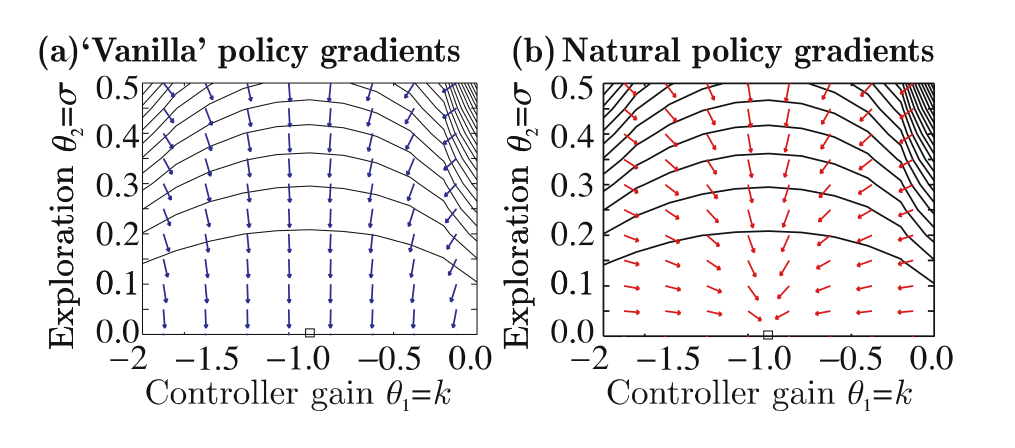
\includegraphics[width=\textwidth]{nat-grad-adv}
  \caption{An experiment showing where the natural gradient has a great advantage. \cite{Peters_IICHR_2003} }\label{fig:nat-grad-adv}
\end{figure}

Using the Fisher information matrix $F_\theta$, and the gradient estimate we discussed in section \ref{sec:pge} gives us the definition
\begin{equation}
  \widetilde{\nabla}_\theta J(\theta) := F^{-1}_\theta \nabla_\theta J(\theta)
  \label{eqn:nat-grad}
\end{equation}
of the natural gradient. The Fisher information matrix represents the certainty we have on our estimate of the gradient and is defined as the covariance of the log likelihood function of a trajectory $\tau_{\pi_\theta}^h$, which as \cite{4863} show can be written as 
\begin{equation}
  F_\theta = \int_\mathbb{S} p(s|\theta) \int_\mathbb{A} \pi_\theta(a|s) \nabla_\theta \log{\pi_\theta(a|s)} \nabla_\theta \log{\pi_\theta(a|s)}^T dads.
  \label{eqn:F}
\end{equation}
When we recall the definition \eqref{eqn:like-grad} of likelihood-ratio gradients, we see that setting $\psi$ as $\nabla_\theta \log \pi(a|s)^T w$, we get
\begin{equation}
  \nabla_\theta J(\theta) = \int_\mathbb{S} {p(s|\theta) \int_\mathbb{A} \pi_\theta(a|s) \nabla_\theta \log \pi(a|s) {\nabla_\theta \log \pi(a|s)}^T dads}\ w := F_\theta w.
  \label{eqn:J-equals-F}
\end{equation}

From \eqref{eqn:nat-grad}, \eqref{eqn:F}, and \eqref{eqn:J-equals-F}, it follows that
\begin{equation}
  \widetilde{\nabla}_\theta J(\theta) = F^{-1}_\theta \nabla_\theta J(\theta) = F_\theta^{-1} F_\theta w = w.
\end{equation}
Thus, this approach does not require an actual estimate of the Fisher information matrix, but only an estimate of $w$, with the update step according to $\theta_{k+1} = \theta_k + \alpha_k w$.

Peters et al. \cite{4863} present this idea and suggest LSTD($\lambda$)-Q, a version of least-squares temporal difference learning  \cite{Boyan:1999:LTD:645528.657618}, as well as episodic natural actor-critic.

Note that this approach abuses some specific conveniences about the problem setup to find an elegant solution. However, this is not the only way to approach this problem. In this paper, we focus on one presentation to present the core idea, but the field of policy gradient optimization is very resourceful. TODO In the conclusion \ref{sec:outro}, we attempt to show the versatility and relevance in current research, and give some directions for further reading.

\section{Conclusion}
\label{sec:outro}

TODO less references and stuff...

In this paper, we have introduced policy gradient methods as a class of reinforcement learning algorithms. We show why policy gradient methods are effective in these environments, and we give some intuitions about the concept. Further, we show the core elements of policy gradient methods, and we discuss some intricacies that they bring, and some research development in the attempts of improving the efficiency and stability of policy gradients.

There are many possibilities for improvement as it can be seen as a very modularized and flexible. We find that the theoretical basis for policy gradient focused approaches reaches far back with some fundamental algorithms like Levenberg-Marquardt \cite{levenbergmarquardt1978}, and the first presentation of REINFORCE \cite{Williams92simplestatistical}. Policy gradient methods were shown to be increasingly potent by authors such as Sutton \cite{Sutton:1999:PGM:3009657.3009806}, and still provide space for a lot of new work being published. Algorithms such as the aforementioned Natural Actor-Critic \cite{4863} have been showing some of their potentials, but even so potential areas of improvement. Schulman et al. \cite{DBLP:journals/corr/SchulmanMLJA15} present a form of advantage estimation using $\gamma$ as a parameter for bias-variance trade-off. Fellows et al. \cite{fellows:icml18} use Fourier analysis to analytically improve policy gradients. Abdolmaleki et al. \cite{abdolmaleki2018maximum} introduce MPO, an off-policy algorithm using expectation maximization, related to the approach of TRPO \cite{pmlr-v37-schulman15}. Yet a different approach is given by Zhang et al. \cite{DBLP:journals/corr/abs-1808-03030}, who formulate policy optimization as a Wasserstein gradient flow problem, which moves into a Wasserstein manifold in the distribution space. This is comparable to approaches by Abdolmaleki et al. \cite{NIPS2015_5672}, which introduces a bound on the Kullback-Leibler divergence during policy search. From the developments in recent research, it is fair to say that policy gradient methods play a major role in reinforcement learning. 

\bibliographystyle{spmpsci}
\bibliography{bibliography}

\end{document}
